\documentclass[a4paper,12pt]{article}

\usepackage{graphicx}
\usepackage{caption}
\usepackage{subcaption}
\usepackage{tikz}
\usepackage{pgf}
\usepackage{amsmath}
\usetikzlibrary{arrows.meta}
\usepackage[utf8]{inputenc}
\usepackage[english,greek]{babel}
\usepackage{hyperref}

\title{Τεχνικές Βελτιστοποίησης - \selectlanguage{english} Project 2024}
\author{Ρουσομάνης Γεώργιος (ΑΕΜ: 10703)}
\date{Ιανουάριος 2025}

\begin{document}

\maketitle

\section*{Εισαγωγή}

Σε αυτήν την εργασία καλούμαστε να δημιουργήσουμε έναν γενετικό αλγόριθμο που θα ελαχιστοποιεί μία συνάρτηση 
πολλών μεταβλητών η οποία θα υπόκεινται σε γραμμικούς ισοτικούς και ανισοτικούς περιορισμούς.

Θεωρούμε το οδικό δίκτυο του Σχ.~\ref{fig:traffic_network}, όπου οι κόμβοι παριστάνουν οδικές διασταυρώσεις 
και τα βέλη κυκλοφοριακές κατευθύνσεις. Οι αριθμοί με μαύρο χρώμα ορίζουν την αρίθμηση των δρόμων/ακμών, ενώ οι
αριθμοί με κόκκινο ορίζουν τον μέγιστο δυνατό ρυθμό διέλευσης οχημάτων σε κάθε δρόμο. Ο χρόνος κίνησης στον δρόμο
$i$ συναρτήσει του ρυθμού διέλευσης των οχημάτων $x_i$ είναι:
\begin{equation}
T_i(x_i) = t_i + \alpha_i \frac{x_i}{1 - \frac{x_i}{c_i}}[\text{\selectlanguage{english}min}],
\label{eq:road_travel_time}
\end{equation}
όπου $t_i$ ο σταθερός χρόνος που απαιτείται για να κινηθούμε στο δρόμο $i$ όταν η κίνηση είναι ασθενής, $c_i$
ο μέγιστος δυνατός ρυθμός διέλευσης οχημάτων από τον ίδιο δρόμο και 
$\alpha_i = 1.25, \, i=1,...,5, \, \alpha_i = 1.5, \, i = 6,...,10, \, \alpha_i = 1, \, i = 11,...,17$.

Επιθυμούμε να ελαχιστοποιήσουμε ως προς $x_i$ τον συνολικό χρόνο διάσχισης του δικτύου του 
Σχ.~\ref{fig:traffic_network} ανά όχημα για ρυθμό εισερχόμενων οχημάτων ίσο με 
$V[$οχ.$/\text{\selectlanguage{english}min}]$. Για να αποφύγουμε τη συγκέντρωση οχημάτων 
στους κόμβους του δικτύου, είναι επιθυμητό όσα οχήματα εισέρχονται σε κάθε κόμβο τόσα και να εξέρχονται.

\newpage

\begin{figure}[htbp]
    \centering
    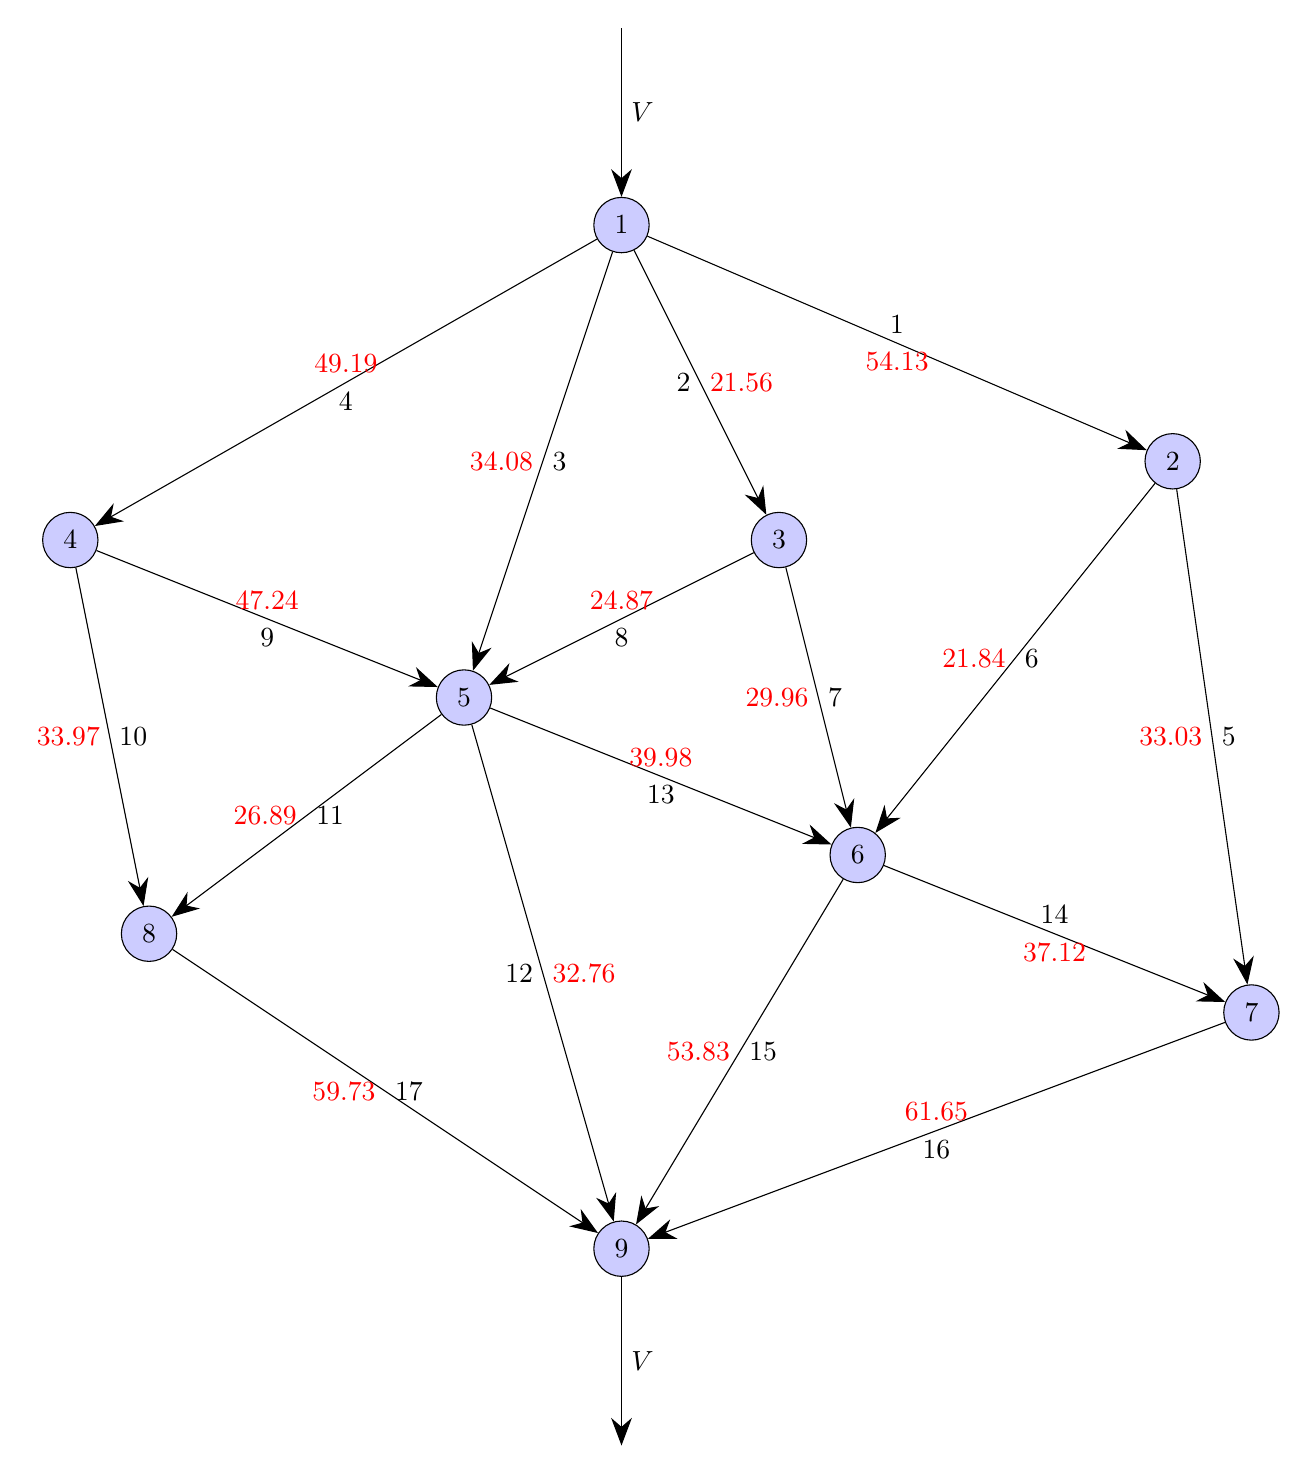
\begin{tikzpicture}[
        xshift=-2cm,  % Shifts the entire figure 2cm to the left
        > = {Stealth[length=10pt]},
        vertex/.style = {circle, draw, fill=blue!20, minimum size=20pt},
        every edge/.style = {draw, ->, thick}
    ]
        % Nodes with increased spacing
        \node[vertex] (v1) at (0,10) {1};
        \node[vertex] (v2) at (7,7) {2};
        \node[vertex] (v3) at (2,6) {3};
        \node[vertex] (v4) at (-7,6) {4};
        \node[vertex] (v5) at (-2,4) {5};
        \node[vertex] (v6) at (3,2) {6};
        \node[vertex] (v7) at (8,0) {7};
        \node[vertex] (v8) at (-6,1) {8};
        \node[vertex] (v9) at (0,-3) {9};

        % Added entry point above node 1
        \draw[->] (0,12.5) -- (v1) node[midway, right] {$V$};
        
        % Added exit point below node 9
        \draw[->] (v9) -- (0,-5.5) node[midway, right] {$V$};
        
        % Edges with centered labels on opposite sides
        \draw[->] (v1) -- (v2) node[midway, above] {1} node[midway, below, red] {54.13};
        \draw[->] (v1) -- (v3) node[midway, left] {2} node[midway, right, red] {21.56};
        \draw[->] (v1) -- (v5) node[midway, right] {3} node[midway, left, red] {34.08};
        \draw[->] (v1) -- (v4) node[midway, below] {4} node[midway, above, red] {49.19};
        \draw[->] (v2) -- (v7) node[midway, right] {5} node[midway, left, red] {33.03};
        \draw[->] (v2) -- (v6) node[midway, right] {6} node[midway, left, red] {21.84};
        \draw[->] (v3) -- (v6) node[midway, right] {7} node[midway, left, red] {29.96};
        \draw[->] (v3) -- (v5) node[midway, below] {8} node[midway, above, red] {24.87};
        \draw[->] (v4) -- (v5) node[midway, below] {9} node[midway, above, red] {47.24};
        \draw[->] (v4) -- (v8) node[midway, right] {10} node[midway, left, red] {33.97};
        \draw[->] (v5) -- (v8) node[midway, right] {11} node[midway, left, red] {26.89};
        \draw[->] (v5) -- (v9) node[midway, left] {12} node[midway, right, red] {32.76};
        \draw[->] (v5) -- (v6) node[midway, below] {13} node[midway, above, red] {39.98};
        \draw[->] (v6) -- (v7) node[midway, above] {14} node[midway, below, red] {37.12};
        \draw[->] (v6) -- (v9) node[midway, right] {15} node[midway, left, red] {53.83};
        \draw[->] (v7) -- (v9) node[midway, below] {16} node[midway, above, red] {61.65};
        \draw[->] (v8) -- (v9) node[midway, right] {17} node[midway, left, red] {59.73};
    \end{tikzpicture}
    \caption{Οδικό δίκτυο}
    \label{fig:traffic_network}
\end{figure}

\newpage

\section{Μαθηματική διατύπωση του προβλήματος}

Η συνάρτηση που καλούμαστε να ελαχιστοποιήσουμε είναι η
\begin{equation}
f(x_1,...,x_{M}) = \sum_{i=1}^{M}\alpha_i \frac{x_i}{1 - \frac{x_i}{c_i}}
\label{eq:objective}
\end{equation}
όπου $M$ το πλήθος των ακμών, υπό τους περιορισμούς
\begin{equation}
0 \leq x_i < c_i, \quad i = 1,...,M.
\label{eq:inequality_constraints}
\end{equation}
Να σημειωθεί ότι στον ορισμό της (\ref{eq:objective}) δεν λάβαμε υπόψη τους όρους $t_i$ της 
(\ref{eq:road_travel_time}) διότι είναι σταθεροί και δεν επηρεάζουν την τελική λύση.
Επίσης, από την απαίτηση για διατήρηση της ροής των οχημάτων σε κάθε κόμβο, πρέπει να ισχύει
\begin{equation}
\sum_{x_i\in E_j^{in}}x_i = \sum_{x_i \in E_j^{out}} x_i, \quad j = 1,...,N,
\label{eq:equality_constraints}
\end{equation}
όπου $E_j^{in}$ και $E_j^{out}$ το σύνολο των εισερχόμενων και εξερχόμενων ροών οχημάτων στον κόμβο $j$
και $N$ το πλήθος των κόμβων.

Προκειμένου να γράψουμε σε μία πιο συμπαγή μορφή την σχέση (\ref{eq:equality_constraints}), 
μοντελοποιούμε το οδικό δίκτυο του Σχ.~\ref{fig:traffic_network} μέσω ενός πίνακα γειτνίασης 
$G_{N\text{\selectlanguage{english}x}N}$ όπου το στοιχείο  $g_{ij}$ δηλώνει τον αριθμό της ακμής που έχει 
αφετηρία τον κόμβο $i$ και τέρμα τον κόμβο $j$. Αν $g_{ij} = 0$ σημαίνει ότι οι κόμβοι $i, j$ δεν ενώνονται
απευθείας μέσω κάποιας ακμής. Συνεπώς, για να βρούμε τις εξερχόμενες ακμές από κάποιο κόμβο $j$ αρκεί να 
διατρέξουμε τα στοιχεία της γραμμής $j$ ενώ για να βρούμε τις εισερχόμενες ακμές αρκεί να διατρέξουμε τα 
στοιχεία της στήλης $j$.

Ορίζουμε τώρα τον πίνακα $A_{N\text{\selectlanguage{english}x}M}$ του οποίου τα στοιχεία δίνονται από:
\begin{equation}
\alpha_{ij} = 
\begin{cases}
1, & \text{\selectlanguage{english}if } j=g_{ik} > 0 \\
-1, & \text{\selectlanguage{english}if } j=g_{li} > 0 \\
0, & \text{\selectlanguage{english}otherwise} 
\end{cases}
\label{eq:A_matrix_definition}
\end{equation}
όπου οι δείκτες $l,k=1,...,N$ διατρέχουν την $i$-οστή γραμμή και στήλη του πίνακα $G$ προκειμένου να εντοπίσουν ποιες 
ακμές εξέρχονται από τον κόμβο $i$ και ποιες εισέρχονται σε αυτόν. Να σημειωθεί ότι εφόσον έχουμε
κατευθυνόμενο γράφο, αν $g_{ik} > 0$ τότε $g_{ki} = 0$ και το αντίστροφο. Με λίγα λόγια, δεν υπάρχουν ακμές
μεταξύ δύο κόμβων που να επιτρέπουν την ροή οχημάτων και προς τις δύο κατευθύνσεις. Συνεπώς, ο μαθηματικός 
φορμαλισμός που χρησιμοποιείται για τον πίνακα $A$ είναι έγκυρος.

Επομένως, η σχέση (\ref{eq:equality_constraints}) μπορεί να γραφτεί σε μορφή πινάκων ως:
\begin{equation}
    A x = b, \quad b = [V,0,...,0,-V]^T
    \label{eq:equality_constraints_matrix_form}
\end{equation}

\newpage

\section{Υλοποίηση Γενετικού Αλγορίθμου}

Θα δημιουργήσουμε έναν εξελικτικό αλγόριθμο ο οποίος θα ελαχιστοποιεί ως προς $x_i$ τον συνολικό χρόνο διάσχισης 
του δικτύου ανά όχημα. Θεωρούμε έναν πληθυσμό από άτομα (χρωμοσώματα), καθένα από τα οποία παριστάνει μία λύση του
προβλήματος βελτιστοποίησης. Τα άτομα αυτά είναι κωδικοποιημένα στη μορφή που βρίσκονται, γι' αυτό και πρόκειται 
ουσιαστικά για μία εξελικτική στρατηγική. 

Ο αλγόριθμος αποτελείται από τα εξής στάδια: 
α) επιλογή αρχικού πληθυσμού που να ικανοποιεί τους περιορισμούς των (\ref{eq:inequality_constraints}) και 
(\ref{eq:equality_constraints}),
β) επιλογή των γονέων οι οποίοι θα δημιουργήσουν τους απογόνους
\selectlanguage{english}(offspring)\selectlanguage{greek},
γ) εφαρμογή του τελεστή διασταύρωσης \selectlanguage{english}(crossover)\selectlanguage{greek} στους γονείς 
για τη δημιουργία των απογόνων και έπειτα εφαρμογή του τελεστή μετάλλαξης σε ένα υποσύνολο των απογόνων και
δ) επιλογή των ατόμων που θα διαμορφώσουν την επόμενη γενιά. 
Τα βήματα αυτά εκτελούνται σε κάθε γενιά (επανάληψη) $k$ του αλγορίθμου και περιγράφονται αναλυτικά στη συνέχεια.
Ο αλγόριθμος τερματίζει όταν συμπληρωθεί ένας προκαθορισμένος αριθμός επαναλήψεων, όπως έχει οριστεί από τον χρήστη.

\subsection{Επιλογή αρχικού πληθυσμού}
Λόγω των ισχυρών περιορισμών που εισάγει το πρόβλημα βελτιστοποίησης, είναι αναγκαία η δημιουργία μίας μεθόδου
που θα δημιουργεί με συστηματικό τρόπο ένα αρχικό εφικτό σύνολο λύσεων. Έστω $\phi_i, i=1,...,N-1$ η καθαρή ροή 
\selectlanguage{english}(net flow)\selectlanguage{greek} των οχημάτων σε κάθε κόμβο, εκτός του τελευταίου, 
σε κάθε επανάληψη της μεθόδου. Είναι προφανές ότι για να είναι ένα σημείο εφικτό θα πρέπει να ισχύει 
$\phi_i = 0, i=1,...,N-1$ κατά τον τερματισμό του αλγορίθμου.

Η μέθοδος ξεκινάει θέτοντας $\phi_1 = V, \phi_i = 0, i=2,...,N-1$. Έπειτα επισκέπτεται διαδοχικά 
τους κόμβους του δικτύου (με την σειρά αρίθμησης που φαίνεται στο Σχ.~\ref{fig:traffic_network}) και για κάθε έναν
από αυτούς κατανέμει την εισερχόμενη σε αυτόν ροή οχημάτων $\phi_i$ στις εξερχόμενες ακμές με τυχαίο τρόπο αλλά 
ικανοποιώντας τους περιορισμούς. 

Να σημειωθεί ότι η αρίθμηση των κόμβων έγινε με τέτοιο τρόπο ώστε όταν ο αλγόριθμος βρίσκεται σε έναν κόμβο $i$, 
να μην υπάρχει εφικτή διαδρομή από κάποιον κόμβο $j > i$ προς τον $i$. Έτσι εξασφαλίζουμε ότι δεν 
υπάρχει εισερχόμενη ροή στον κόμβο $i$ που δεν την έχουμε λάβει υπόψη και επικεντρωνόμαστε στο μηδενισμό του 
$\phi_i$. Η αρίθμηση αυτή είναι γνωστή και ως τοπολογική διάταξη \selectlanguage{english}(topological
ordering)\selectlanguage{greek} του κατευθυνόμενου άκυκλου γράφου\selectlanguage{english}
(Directed Acyclic Graph - DAG)\selectlanguage{greek}. Αν για κάποιο κόμβο $i$ ισχύει ότι η εισερχόμενη ροή είναι 
μεγαλύτερη από τη συνολική μέγιστη χωρητικότητα των ακμών που εξέρχονται από αυτόν, τότε το άτομο απορρίπτεται 
και ο αλγόριθμος ξεκινάει από την αρχή. Ευνόητο είναι ότι όσο μεγαλύτερη είναι η τιμή του $V$, τόσο μεγαλύτερο θα 
είναι και το πλήθος των απορρίψεων.

\subsection{Επιλογή γονέων}
Η επιλογή των γονέων από κάποιον πληθυσμό μπορεί να γίνει με τους εξής τρόπους:
\begin{itemize}
    \item \textbf{Μέθοδος Τουρνουά \selectlanguage{english}(Tournament Method)\selectlanguage{greek}}:
    Από τον αρχικό πληθυσμό επιλέγονται τυχαία $k$ άτομα και από αυτά επιλέγεται ως γονέας το άτομο
    με τη μεγαλύτερη τιμή ικανότητας \selectlanguage{english}(fitness value)\selectlanguage{greek}.
    Επειδή έχουμε πρόβλημα ελαχιστοποίησης, επιλέγεται ως γονέας το άτομο που δίνει τη μικρότερη τιμή
    της αντικειμενικής συνάρτησης. 
    
    Μεγάλες τιμές του $k$, οδηγούν στην επιλογή ανταγωνιστικότερων γονέων
    και σε ταχύτερη σύγκλιση του αλγορίθμου. Ωστόσο υπάρχει ο κίνδυνος πρόωρης σύγκλισης σε κάποιο τοπικό
    ελάχιστο. Αντιθέτως, για μικρές τιμές του $k$ η επιλογή των γονέων γίνεται σχεδόν τυχαία οδηγώντας σε 
    αργή σύγκλιση.

    \item \textbf{Μέθοδος της Ρουλέτας \selectlanguage{english}(Roulette Method)\selectlanguage{greek}}:
    Στη ρουλέτα, κάθε άτομο έχει πιθανότητα επιλογής ανάλογη με την καταλληλότητά του. Αν $f_i$ είναι η
    τιμή της αντικειμενικής συνάρτησης του ατόμου $i$ τότε η καταλληλότητά του θα δίνεται από:
    \begin{equation}
        q_i = f_{max} - f_i + 1,
        \label{eq:roulette_goodness_value}
    \end{equation}
    όπου $f_{max}$ η μέγιστη τιμή της αντικειμενικής συνάρτησης του πληθυσμού. Βλέπουμε ότι μικρότερες τιμές
    $f_i$ οδηγούν σε μεγαλύτερες τιμές καταλληλότητας. Η μονάδα στην (\ref{eq:roulette_goodness_value}) προστίθεται
    ώστε να μην υπάρχουν άτομα με μηδενική πιθανότητα επιλογής, διατηρώντας την ποικιλομορφία του πληθυσμού.
    Η πιθανότητα εμφάνισης του ατόμου $i$ δίνεται από:
    \begin{equation}
        p_i = \frac{q_i}{\sum_{j=1}^{M}q_j}
        \label{eq:roulette_selection_probability}
    \end{equation}

    Το πλεονέκτημα της μεθόδου είναι ότι διατηρεί τη διαφορετικότητα του πληθυσμού, καθώς ακόμα και άτομα με χαμηλή 
    καταλληλότητα έχουν πιθανότητα επιλογής. Ωστόσο είναι υπολογιστικά πιο απαιτητική σε σύγκριση με τη μέθοδο τουρνουά.

    \item \textbf{Τυχαία Επιλογή \selectlanguage{english}(Random Selection)\selectlanguage{greek}}:
    Η μέθοδος αυτή επιλέγει τους γονείς εντελώς τυχαία, χωρίς να λαμβάνει υπόψη την καταλληλότητά τους.

    Στα πλεονεκτήματά της είναι η διατήρηση υψηλής ποικιλομορφίας στον πληθυσμό, αποφεύγοντας την πρόωρη σύγκλιση,
    ενώ είναι απλούστερη και ταχύτερη σε υπολογιστική πολυπλοκότητα από όλες τις άλλες μεθόδους. Το μειονέκτημά της
    είναι ο χαμηλός ρυθμός σύγκλισης ενώ ενδέχεται η εξέλιξη να γίνει αναποτελεσματική, αφού δεν ευνοούνται οι πιο 
    κατάλληλες λύσεις.
    
\end{itemize}

Στο Σχ.~\ref{fig:genetic_convergence} απεικονίζεται η σύγκλιση του γενετικού αλγόριθμου για τις τρεις μεθόδους
επιλογής γονέων ενώ παράλληλα παρατίθεται και η λύση της συνάρτησης \selectlanguage{english}fmincon\selectlanguage{greek}
του \selectlanguage{english}MATLAB\selectlanguage{greek} για λόγους σύγκρισης.
Στο Σχ.~\ref{fig:genetic_distance} παρατηρούμε ότι οι λύσεις και των τριών μεθόδων έχουν την τάση να συγκλίνουν 
προς τη λύση της \selectlanguage{english}fmincon\selectlanguage{greek}.

\begin{figure}[h]
    \centering
    \begin{minipage}{0.45\textwidth}
        \centering
        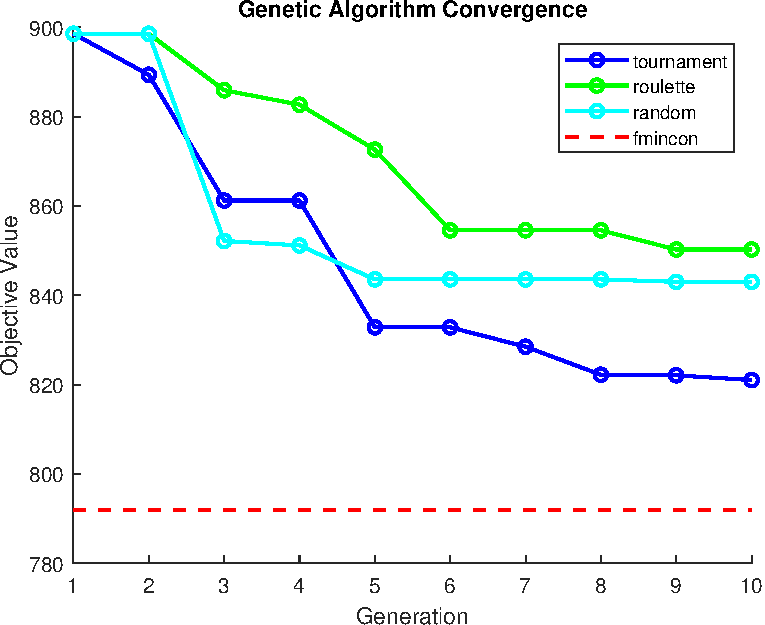
\includegraphics[width=\linewidth]{plot/genetic_convergence.pdf}
        \caption{Σύγκλιση γενετικού αλγορίθμου για διάφορες μεθόδους επιλογής γονέων}
        \label{fig:genetic_convergence}
    \end{minipage}
    \hfill
    \begin{minipage}{0.45\textwidth}
        \centering
        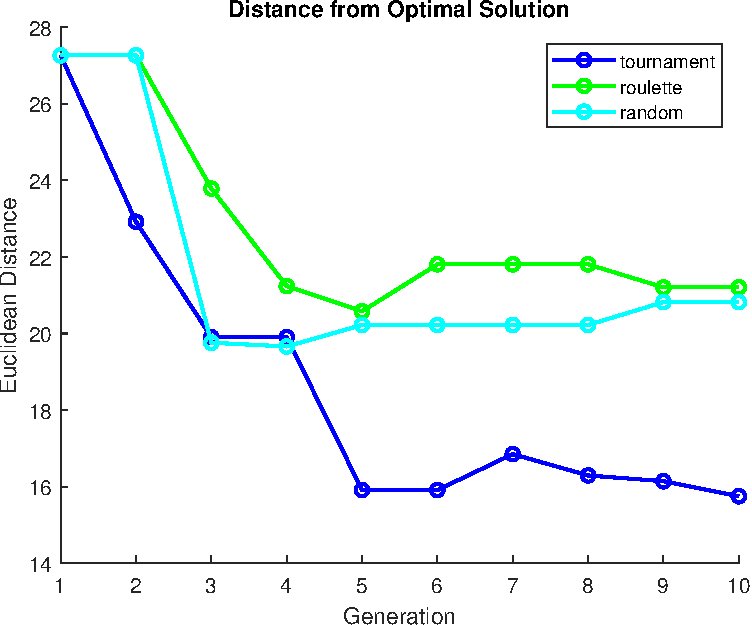
\includegraphics[width=\linewidth]{plot/genetic_distance.pdf}
        \caption{Ευκλείδια απόσταση της λύσης του γενετικού αλγορίθμου από την λύση της συνάρτησης 
        \selectlanguage{english}fmincon\selectlanguage{greek} του \selectlanguage{english}MATLAB\selectlanguage{greek}}
        \label{fig:genetic_distance}
    \end{minipage}
\end{figure}

\subsection{Δημιουργία απογόνων και μετάλλαξη}
Έχοντας επιλέξει τους δύο γονείς με μία από τις παραπάνω στρατηγικές, εφαρμόζουμε τον τελεστή διασταύρωσης
\selectlanguage{english}(crossover)\selectlanguage{greek} σε αυτούς για να προκύψει ένας απόγονος. 
Αν $p_1$ και $p_2$ είναι οι δύο γονείς, ο απόγονός τους θα δίνεται από τον σταθμισμένο γραμμικό συνδυασμό τους ως:
\begin{equation}
    x = \gamma p_1 +(1 - \gamma) p_2, \quad 0 < \gamma < 1,
    \label{eq:crossover}
\end{equation}
όπου η σταθερά $\gamma$ επιλέγεται τυχαία κάθε φορά. 

Αν ο απόγονος που προκύπτει δεν ικανοποιεί τους περιορισμούς
των (\ref{eq:inequality_constraints}) και (\ref{eq:equality_constraints_matrix_form}), επιλέγονται εκ νέου οι γονείς
και εφαρμόζεται ξανά η (\ref{eq:crossover}). Η διαδικασία επαναλαμβάνεται έως ότου προκύψει ένας εφικτός απόγονος ή
ξεπεραστεί ο μέγιστος αριθμός επαναλήψεων. Να σημειωθεί ότι ο έλεγχος της (\ref{eq:equality_constraints_matrix_form})
προγραμματιστικά γίνεται με ένα επίπεδο ανοχής $\epsilon > 0$, δηλαδή ικανοποιείται αν $|Ax - b| < \epsilon$.

Για τη δημιουργία των απογόνων χρησιμοποιήθηκε η τεχνική του σταθμισμένου γραμμικού συνδυασμού και όχι η διακριτή
διασταύρωση. Ο λόγος είναι ότι στη δεύτερη μέθοδο, οι απόγονοι κληρονομούν ένα τμήμα από τον έναν γονέα και ένα από τον
άλλο, γεγονός που καθιστά εξαιρετικά απίθανο να ικανοποιηθεί η (\ref{eq:equality_constraints_matrix_form}), με 
αποτέλεσμα να αποτρέπεται η εξέλιξη του πληθυσμού.

Έστω $\Theta_k$ το σύνολο των απογόνων και $\Omega_k$ το σύνολο του πληθυσμού από το οποίο προέκυψαν οι απόγονοι
στην γενιά (επανάληψη) $k$. Το μέγεθος του $\Theta_k$ ελέγχεται μέσω μίας υπερπαραμέτρου 
\selectlanguage{english}(hyperparameter)\selectlanguage{greek} $\lambda$ σύμφωνα με την σχέση:
\begin{equation}
    |\Theta_k| = \lambda |\Omega_k|, \quad 0 < \lambda < 1
    \label{eq:population_offspring_size}
\end{equation}
Διαλέγουμε τυχαία ένα υποσύνολο $\bar{\Theta}_k$ του $\Theta_k$, 
προκειμένου να εφαρμόσουμε τον τελεστή της μετάλλαξης. Το μέγεθος του $\bar{\Theta}_k$ ελέγχεται και πάλι μέσω μίας
υπερπαραμέτρου $\mu$ σύμφωνα με την σχέση:
\begin{equation}
    |\bar{\Theta}_k| = \mu |\Theta_k|, \quad 0 < \mu < 1
    \label{eq:offspring_mutation_size}
\end{equation}
Μέτα τη μετάλλαξη, κάθε όρισμα του ατόμου δίνεται από:
\begin{equation}
    x_i(k) = x_i(k-1) + \Delta x_i,
    \label{eq:mutation}
\end{equation}
Στην υλοποίησή μας θεωρούμε την απλουστευμένη περίπτωση όπου τα $\Delta x_i$ ακολουθούν όλα την ίδια Γκαουσιανή 
κατανομή με μέση τιμή μηδέν και τυπική απόκλιση $\sigma$. 

Όπως και στην περίπτωση της διασταύρωσης, η (\ref{eq:mutation}) επαναλαμβάνεται έως ότου προκύψει εφικτό σημείο
ή ξεπεραστεί ο μέγιστος αριθμός επαναλήψεων. Μεγάλες τιμές του $\sigma$ οδηγούν σε πιο βίαιες αποκλίσεις από
τοπικά ελάχιστα αλλά και σε μεγαλύτερα ποσοστά απόρριψης των μεταλλάξεων λόγω μη ικανοποίησης των περιορισμών.

\subsection{Δημιουργία νέας γενιάς}
Η διαδικασία επιλογής των ατόμων που θα απαρτίζουν την νέα γενιά γίνεται κατά ντετερμινιστικό τρόπο. Από την
(\ref{eq:population_offspring_size}), ο πληθυσμός της επόμενης γενιάς, $\Omega_{k+1}$, θα αποτελείται κατά το
ποσοστό $\lambda$ από τους απογόνους και κατά $1 - \lambda$ από τα άτομα της προηγούμενης γενιάς με τη μικρότερη
τιμή της αντικειμενικής συνάρτησης.

Τιμές του $\lambda$ κοντά στην μονάδα προσδίδουν πιο έντονα το χαρακτήρα της ολικής αναζήτησης. Η πλειοψηφία των
γονέων πεθαίνουν σε κάθε γενιά και η επιλογή γίνεται κατά κύριο λόγο ανάμεσα στους απογόνους. Με αυτόν τον τρόπο 
ενισχύεται η προσαρμοστικότητα και η ευρύτητα του χώρου αναζήτησης με κίνδυνο ωστόσο να χαθούν ορισμένες καλές,
μέχρι εκείνη τη στιγμή, λύσεις.

Αντίθετα, τιμές του $\lambda$ κοντά στο μηδέν δεν απορρίπτουν τις καλές μέχρι εκείνη την στιγμή λύσεις,
επιτυγχάνοντας ταχύτερη σύγκλιση. Το μειονέκτημα σε αυτή την περίπτωση είναι ότι αν βρεθεί μία καλή λύση,
όλος ο πληθυσμός θα τείνει να συγκεντρωθεί στην γειτονία αυτής.

\section{Μεταβολή του ρυθμού εισερχομένων οχημάτων}

Μέχρι τώρα υποθέταμε ότι ο ρυθμός εισερχομένων οχημάτων $V$ ήταν σταθερός, με τιμή $V = 100$.  
Στην πραγματικότητα, όμως, το $V$ δεν είναι απόλυτα σταθερό αλλά μπορεί να κυμαίνεται σε ένα εύρος τιμών.  

Υποθέτουμε πλέον ότι το $V$ μπορεί να αυξηθεί ή να μειωθεί έως και 15\%.  
Είναι λογικό ότι όσο μεγαλύτερη είναι η κυκλοφορία, τόσο περισσότερος χρόνος απαιτείται  
για τη διάσχιση του δικτύου. Αυτή η συσχέτιση απεικονίζεται στο Σχ.~\ref{fig:solutions_for_different_traffic_flows},  
όπου παρουσιάζουμε και τη λύση που προκύπτει από τη χρήση της συνάρτησης 
\selectlanguage{english}fmincon\selectlanguage{greek} για λόγους σύγκρισης.

Δεδομένου ότι η \selectlanguage{english}fmincon\selectlanguage{greek} υπολογίζει το ολικό ελάχιστο της 
αντικειμενικής συνάρτησης, μπορούμε να προσαρμόσουμε ένα πολυώνυμο δευτέρου βαθμού στα αποτελέσματά της.  
Η προσαρμογή αυτή (μαύρη διακεκομμένη γραμμή στο Σχ.~\ref{fig:solutions_for_different_traffic_flows})  
παρέχει μια πολύ καλή προσέγγιση για τον ελάχιστο χρόνο διάσχισης συναρτήσει του \(V\).

Το πολυώνυμο που περιγράφει αυτή τη σχέση δίνεται από την εξίσωση:
\begin{equation}
    T_{min}(V) = 0.2646V^2 - 33.9056V + 1536.2
    \label{eq:polynomial}
\end{equation}

Στο Σχ.~\ref{fig:/genetic_convergence_inflow_gene} φαίνεται η σύγκλιση του γενετικού αλγορίθμου για κάθε
στρατηγική επιλογής γονέα, \textbf{όπου το $V$ έχει συμπεριληφθεί ως γονίδιο στα χρωμοσώματα}. Σε αντίθεση με τις
προηγούμενες περιπτώσεις, βλέπουμε ότι η \selectlanguage{english}fmincon\selectlanguage{greek} έχει χειρότερη
επίδοση από τον γενετικό αλγόριθμο. Αυτό εξηγείται από το γεγονός ότι ο γενετικός αλγόριθμος έχει προτίμηση
στα χρωμοσώματα με τιμή $V$ κοντά στο 85.
Επιπλέον, λόγω της μεγάλης επιρροής του γονιδίου που αντιστοιχεί στο $V$ για τον καθορισμό του ελαχίστου, η  
\selectlanguage{english}fmincon\selectlanguage{greek} είναι ιδιαίτερα ευαίσθητη στην αρχική επιλογή της τιμής του.
Μια αρχική τιμή του $V$ πολύ υψηλή σε σχέση με το 85 μπορεί να οδηγήσει σε αποτυχία σύγκλισης της 
\selectlanguage{english}fmincon\selectlanguage{greek}.

\begin{figure}[h]
    \centering
    \begin{minipage}{0.45\textwidth}
        \centering
        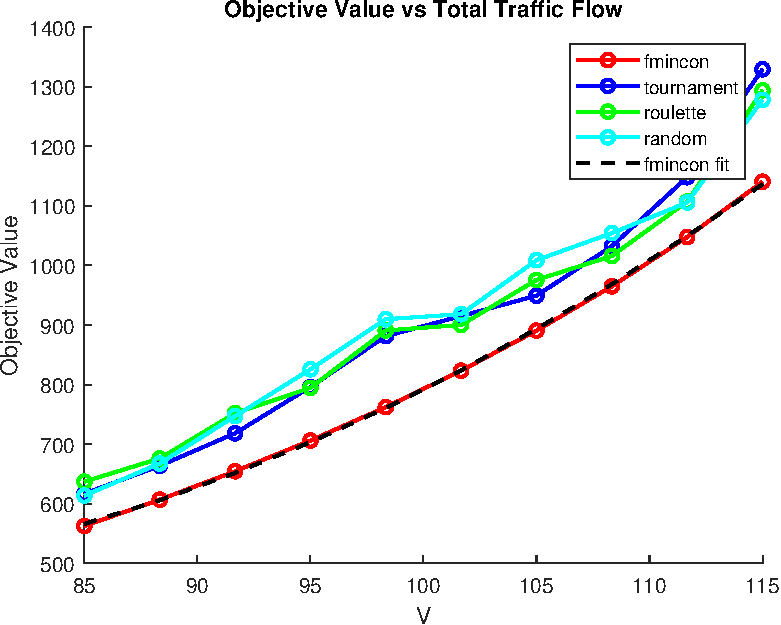
\includegraphics[width=\linewidth]{plot/solutions_for_different_traffic_flows.pdf}
        \caption{Ελάχιστος χρόνος διάσχισης του δικτύου συναρτήσει του ρυθμού εισερχομένων οχημάτων}
        \label{fig:solutions_for_different_traffic_flows}
    \end{minipage}
    \hfill
    \begin{minipage}{0.45\textwidth}
        \centering
        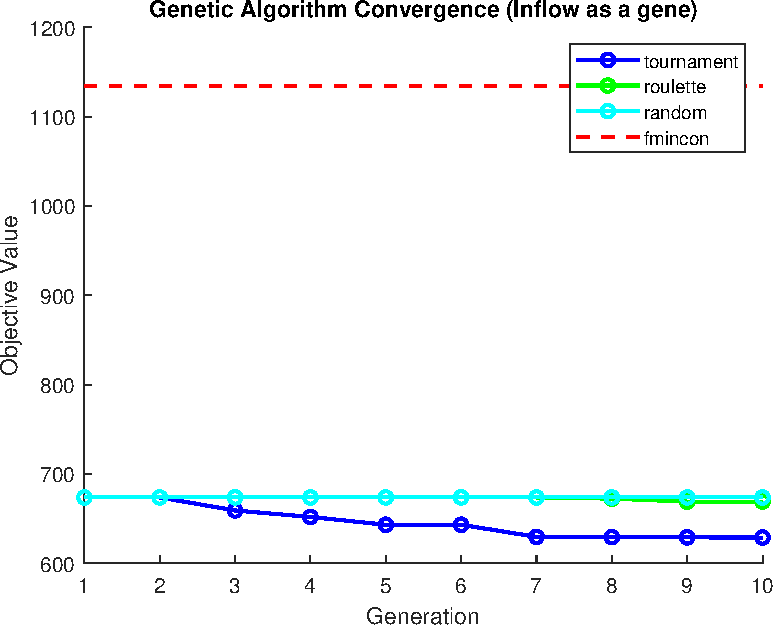
\includegraphics[width=\linewidth]{plot/genetic_convergence_inflow_gene.pdf}
        \caption{Σύγκλιση γενετικού αλγορίθμου για διάφορες μεθόδους επιλογής γονέων με τον ρυθμό εισερχομένων 
        οχημάτων ως γονίδιο των χρωμοσωμάτων}
        \label{fig:/genetic_convergence_inflow_gene}
    \end{minipage}
\end{figure}

\section*{Συμπεράσματα}

Στην παρούσα εργασία μελετήσαμε τη βελτιστοποίηση της ροής οχημάτων σε ένα οδικό δίκτυο χρησιμοποιώντας έναν 
γενετικό αλγόριθμο. Το πρόβλημα διατυπώθηκε μαθηματικά ως ελαχιστοποίηση του συνολικού χρόνου διάσχισης του 
δικτύου, λαμβάνοντας υπόψη περιορισμούς κυκλοφορίας και διατήρησης της ροής των οχημάτων στους κόμβους.

Ο γενετικός αλγόριθμος αναπτύχθηκε με διαδικασίες επιλογής γονέων, διασταύρωσης και μετάλλαξης, διασφαλίζοντας 
τη διατήρηση εφικτών λύσεων. Συγκρίνοντας τις μεθόδους επιλογής γονέων (τουρνουά, ρουλέτα, τυχαία επιλογή), 
διαπιστώθηκε ότι η μέθοδος τουρνουά επιτυγχάνει ταχύτερη σύγκλιση αλλά ενέχει τον κίνδυνο πρόωρης σύγκλισης,
ενώ η ρουλέτα διατηρεί μεγαλύτερη ποικιλομορφία στον πληθυσμό. 

Η σύγκριση του γενετικού αλγορίθμου
με τη μέθοδο \selectlanguage{english}fmincon\selectlanguage{greek} καταδεικνύει ότι ο γενετικός αλγόριθμος αποδίδει
καλύτερα όταν το $V$ ενσωματώνεται ως γονίδιο στο χρωμόσωμα, καθώς προσαρμόζεται δυναμικά σε πιο αποδοτικές 
τιμές. Αντίθετα, η \selectlanguage{english}fmincon\selectlanguage{greek} αποδεικνύεται ευαίσθητη στις αρχικές 
συνθήκες, με υψηλές αρχικές τιμές του $V$ να οδηγούν σε αποτυχία σύγκλισης. 

Συνολικά, η χρήση γενετικού 
αλγορίθμου παρέχει μία αποτελεσματική προσέγγιση για τη βελτιστοποίηση της ροής κυκλοφορίας, εξασφαλίζοντας ευελιξία
και ανθεκτικότητα στις μεταβολές των παραμέτρων του συστήματος.

\end{document}
